\chapter{Fortschreitende Elektronikentwicklung}\label{cha:Elektronikentwicklung}

In diesem Kapitel der Arbeit wird die Umsetzung der diversen Konzept und Strukturanforderungen in Hardware betrachtet. Dabei werden hier ausgesuchte Beispiele aus mehreren Vergangenen Jahren Vorgestellt und Technisch erläutert.
Dabei wird die kontinuierlich Fortschreitende Implementierung von Erfahrung im Zusammenspiel mit dem Modularen Gesamtkonzept aufgezeigt.

\section{Ursprünglicher Elektronikzustand}

Die in der Saison 2014 begonnen Voruntersuchungen fanden mit dem Flugsystem 'Maya' statt.
Abseits von Strukturellen und Flugmechanischen Problemen war auch die Elektronik eine kontinuierliche Quelle von Fehlern und Ausfällen des Flugzeugs.
Dies war größtenteils auf die Mangelnde Erfahrung im Umgang mit einem System eines solchen Komplexitätgrades zurückzuführen.Aber auch eine noch unzureichende Ausstattung mit Werkzeug,  Testmöglichkeiten und Methoden in Kombination mit der Unübersichtlichen Kabelführung erschwerte die Fehlersuche.
Auch die ersten versuche mit einem selbst gebauten Flächenmodell waren mit ähnlichen Schwierigkeiten in der Elektronik behaftet.

\begin{figure}[H]
\centering
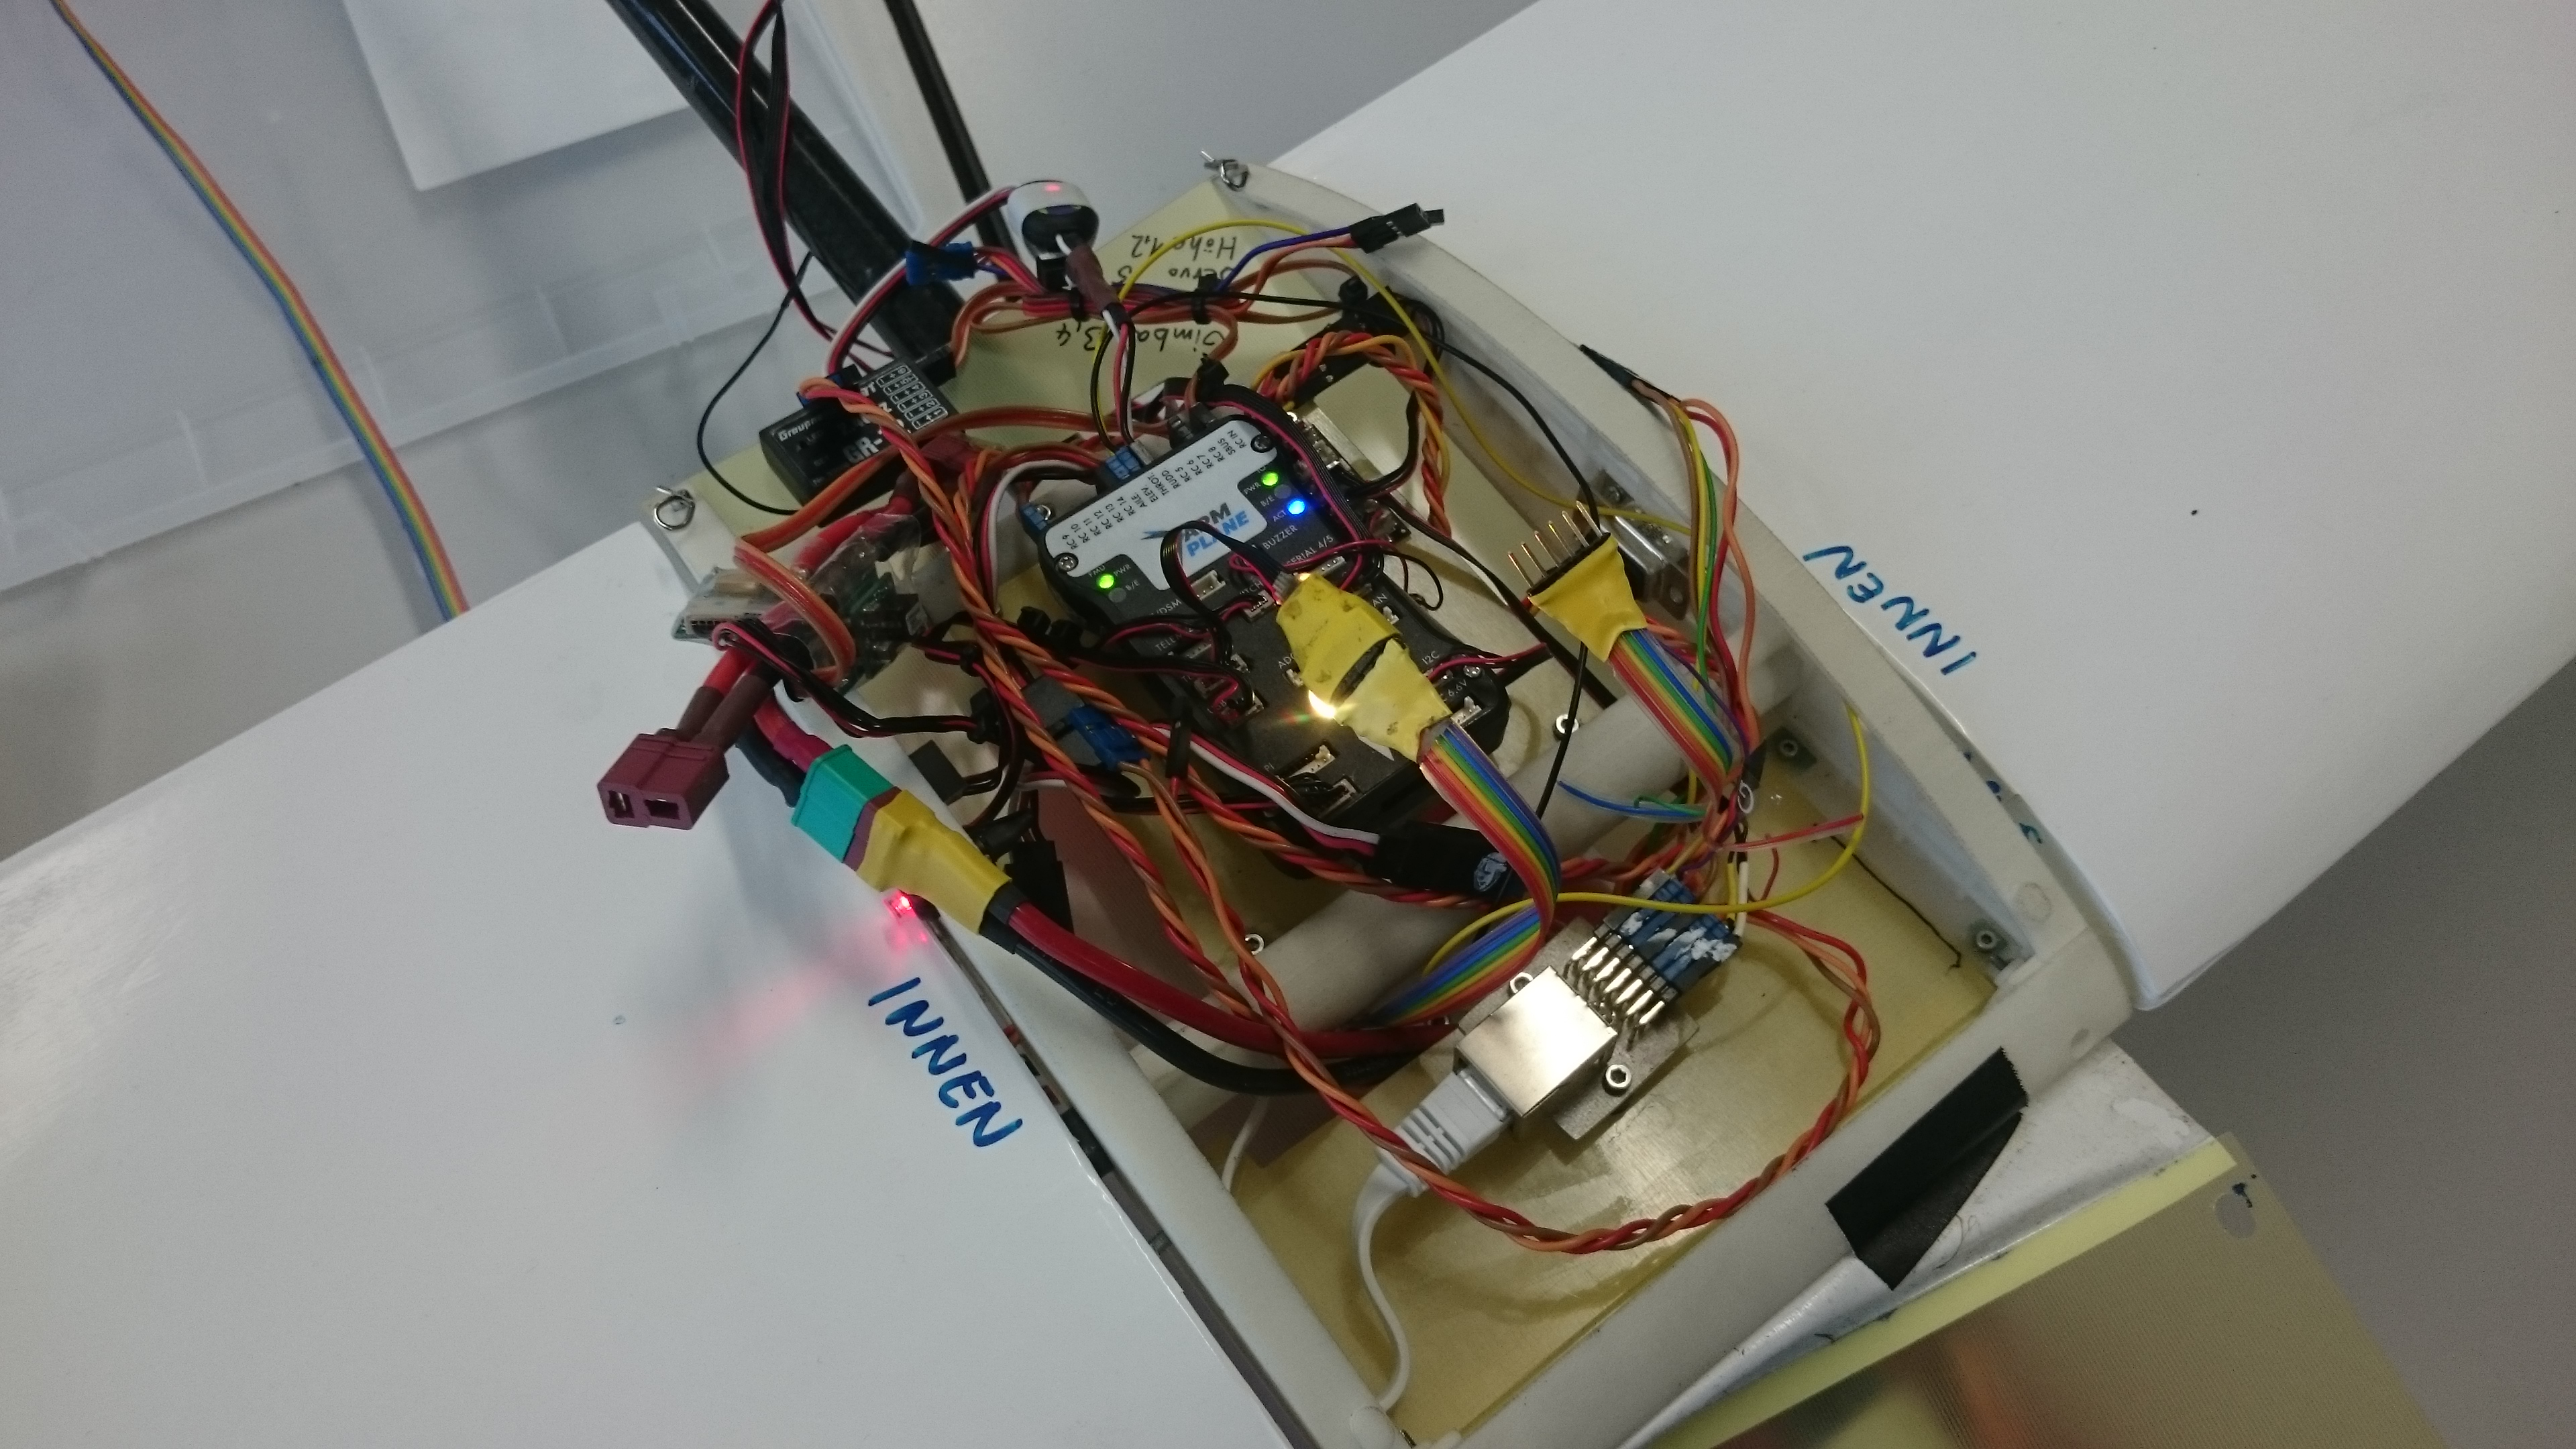
\includegraphics[width=0.9\textwidth]{bilder/Fotos/Elektronik_Kabelsalat_2015.jpg} 
\caption{Anblick der Elektronik zu Beginn 2015} 
\label{Anblick der Elektronik zu Beginn 2015}
\end{figure}

\section{Neue Platinenaufteilung}

Aus diesen Erfahrungen entstand das Eingangs vorgestellte Konzept für die Elektronik des Fliegers.
Dieses Konzept wurde 2015 erstmals angewandt, um eine Übersichtliche und einfach handhabbare Hardwareplattform mit leicht überprüfbaren Funktionen Umzusetzen.

Im Folgenden wird Beispielhaft die Bordelektronik des AUVSI 2016 Fliegers betrachtet.

\subsection{Leistungsplatine}

Die Leistungsplatine kann grundlegend in drei Funktionsgruppen aufgeteilt werden.
Eine Stromrichtungskontrolle in Form der Idealen Dioden Schaltung.
Die Wandlung und Verteilung der Spannungsversorgung für Servos, Sensoren und Autopilotenhardware.
Und eine Priorisierungsschaltung zwischen einem Externen Pfad und der Stromschiene aus dem Zusammenschluss der Idealen Dioden Ausgänge.

Die Idealen Dioden agieren nach dem selben Funktionsprinzip der Idealen Dioden als Modul, auf deren Details in einem späteren Kapitel eingegangen wird. Sie sind an dieser Stelle mit dem IC LTC4352 der Firma Linear Technologys ausgeführt.

Die Spannungsversorgung wird Konzeptgemäß für drei 5\,V Schienen mit Dc-Dc Wandlung aus dem bis zu 17 V Batteriespannung ausgeführt.
Konkret werden zwei Module DSN-360 Mini und ein Modul LM2596 eingesetzt.
Diese Versorgen die Telemetriemodule und LIDAR, die Pixhawk Hardware und die Servo Versorgung.
Die Versorgung der Dc-Dc Module wir an ihrem Eingang mit einem 470\,$\mu$F 25\,V  Elektrolythkondensator gepuffert.

Alle ein und Ausgänge der Module sind mit Selbstrückstellenden Sicherungen der PTC Technologie ausgestattet.

Die Prioritätsschaltung zwischen dem Anschluss den Bodenstromversorgung und dem eigentlich Flugakku wird von einem IC vom Typ LTC4236 gesteuert. Dieser aktuiert drei N-Kanal Mosfets. Einmal in sogenannter 'Back to Back' Konfiguration für den Flugakku Strang und einmal in klassischem Aufbau von Drain nach Source für den Externen Versorger.
Über einen Spannungsteiler detektiert der IC die Präsenz eines Externen Akkus mit einer Spannung größer 14\,V und schaltet daraufhin die Mosfets der Flugenergieversorgung nichtleitend und der externe Mosfet wird auf das Bordsystem durchgeschaltet.
Entsprechend wird bei einem Abfall der Spannung am Externen Anschluss unter 12\,V beziehungsweise einem Entfernen dieses Akkus wird der Strompfad wieder auf die erste Energieversorgung umgeschaltet.

\subsubsection{Schaltplan}

\newpage

\begin{figure}[H]
\centering
\includegraphics[width=1.4\textwidth,angle =90]{bilder/Centerbox/Centerbox-Front-Power_AUVSI16.pdf} 
\caption{Schaltplan der Leistungsplatine} 
\label{fig:Schaltplan der Leistungsplatine}
\end{figure}

\subsubsection{Platinenlayout}

\begin{figure}[H]
\centering
\includegraphics[width=0.9\textwidth]{bilder/Centerbox/Centerbox-Front-Power_AUVSI_2016_rev-01_layout.png} 
\caption{Layout der Leistungsplatine} 
\label{fig:Layout der Leistungsplatine}
\end{figure}

\begin{figure}[H]
\centering
\includegraphics[width=0.9\textwidth]{bilder/Centerbox/Centerbox-Front-Power_AUVSI_2016_rev-01-3D.png} 
\caption{3D Rendering der Leistungsplatine} 
\label{fig:3D Rendering der Leistungsplatine}
\end{figure}

\subsection{Autopilotenplatine}

\subsubsection{Schaltplan}

\newpage

\begin{figure}[H]
\centering
\includegraphics[width=1.25\textwidth,angle =90]{bilder/Centerbox/Centerbox-Rear-Pixhawk_AUVSI16.pdf} 
\caption{Schaltplan der Autopilotenplatine} 
\label{fig:Schaltplan der Autopilotenplatine}
\end{figure}

\subsubsection{Platinenlayout}

\begin{figure}[H]
\centering
\includegraphics[width=0.9\textwidth]{bilder/Centerbox/Centerbox-Rear-Pixhawk_AUVSI_2016_rev-01-layout.png} 
\caption{Layout der Autopilotenplatine} 
\label{fig:Layout der Autopilotenplatine}
\end{figure}

\section{Bedien- und Schutz Konzepte}

\subsection{Eineindeutige Verbinderauswahl}

Für die angepasste Führung von Leistungspfaden und Signalpfaden wurden im Laufe des bisherigen Projekts je zwei verschiedene Steckersysteme eingesetzt.
Die Leistungsverbinder sind lediglich in Plus und Minuspol aufgeteilt und die Korrekte Montage wird über eine Mechanische Kodierung sichergestellt.
Bei den Signalverbindern wird eine mechanische Kodierung über eine einmalige Anzahl an Kontakten angestrebt.So kann in Verbindung mit der konsequenten Beschriftung aller Gegenstellen auf der Platinenseite eine fehlerhafte Montage quasi ausgeschlossen werden. Dabei werden zum teil auch bewusst Steckverbinder mit mehr Kontakten als zu übertragenden signalen ausgewählt um diese Einendeutikeit zu erreichen.

Die Hochstromverbindungen werden stets mit Kabelquerschnitten von 1,5 mm ausgeführt \cite{DIN_VDE_0298}. Der Mantel besteht aus PVC außer in der Nähe von heißen Bauteilen an denen Silikon zum einsatz kommt.
Zu beginn wurden als Hochstromstecker Bauteile des Typs XT60 der Firma hexTronik verwendet.
Diese werden von den meisten Zukaufbaugruppen der Pixhawk Systems verwendet und ermöglichten eine mechanisch kodierte eindeutige Verbindung.
Sie sind für Ströme von 60 Ampere und Spannungen von 120 V freigegeben.
Jedoch waren diese Steckverbinder nur zur Lötmontage vorgesehen. Es wurde die Erfahrung gemacht das die Verbindungen zur Kabelseite immer wieder versagten. Teils wegen Qualitativ ungenügender Lötstellen, teils wegen Brüchen durch Handhabung mit Bewegung des Kabels am Übergang von der Lötstelle zum Kupferkabel am Steifigkeitssprung.

\begin{figure}[H]
\centering
\adjincludegraphics[trim={20cm 8cm 16cm 5cm},width=0.9\textwidth,clip]{bilder/Stecker/Stecker_XT60.jpg}
%\includegraphics[width=0.9\textwidth, center]{bilder/Stecker/Stecker_XT60.jpg} 
\caption{XT60 Hochstromverbinder} 
\label{fig:XT60 Hochstromverbinder}
\end{figure}

Daraufhin wurde ein neues System mit Crimpmontage gesucht.
Hierfür wurde das System POWERPOLE 45 der Firma Anderson Power Products ausgewählt. Die Steckverbinder sind bis zu einem Dauerstrom von 55 Ampere und einer Spannung von 300 V freigegeben.
Die Kabelbrüche wurden mit dem Ersatz der Lötverbidungen durch das Crimpsystem beseitigt. Sie können in den Quadratischen Gehäusen beliebig nebeneinander eingeclipt werden was größere Steckblöcke ermöglicht. Jedoch führte diese variable Montierbarkeit auch immer wieder zu wiedersprüchlicher Montage von Ladekabeln und Akkus bezüglich der Polposition.
Außer einer klaren Standardisierung der Polung wurde bisher noch keine Konzept gefunden Bedienfehler auszuschließen. 

\begin{figure}[H]
\centering
\adjincludegraphics[trim={15cm 12cm 10cm 0},width=0.9\textwidth,clip]{bilder/Stecker/Stecker_Anderson_Powerpol.jpg}
%\includegraphics[width=0.9\textwidth, center]{bilder/Stecker/Stecker_Anderson_Powerpol.jpg} 
\caption{Neuer Verbinder  Powerpol 45} 
\label{fig:Neuer Verbinder  Powerpol 45}
\end{figure}

Beide Systeme verwenden das Prinzip des Kraftschlusses für die Fixierung der Steckverbindung. Die für Montage und Demontage nötigen Kräfte sind jedoch an beengten Stellen im Flieger immer wieder hinderlich bei der Handhabung. Deshalb wird eine Formschlussbasierte Fixierung ähnlich den Signal Steckverbindern erwogen.

Für die Verbindung von Signalleitungen  und Versorgungsleitungen mit kleinen Strömen wurde zu Beginn das Stecksystem MSF der Firma Lumberg verwendet.
Dieses ist für 5 A je Pin bei bis zu 160 V freigegeben. Die Fixierung der Verbindung erfolgt hier über Formschluss in Form einer Lasche im Platinensockel des Verbinders welcher eine Nase am Stecker blockiert. Darüber hinaus besteht noch eine gewisser Kraftschluss über die Kontakte der bei der Demontage der Verbindung oft als unerwünscht hoch eingestuft wurde.

Als Alternative wurden die Verbinder aus der PA Reihe der Firma JST erprobt und mittlerweile in den Einsatz überführt.
Die Stecker sind für 3 A je Pin bei maximal 250 V freigegeben.
Die Fixierung wird auch hier über Formschluss in Gestalt einer Hakennase am Kabelseitigen Stecker realisiert.
Die Verbinder haben sich bisher bewährt, da sie einen guten Kompromiss aus kompakterer Baugröße und guter Handhabung in Montage und Demontage gegenüber den bisher verwendeten MSF Verbindern darstellen.
Die Reduzierte Strombelastbarkeit stellt in der Praxis keinen Nachteil dar.Die Logiksignale bringen nur Ströme im mA Bereich auf und auch die Servoversorgung leitet maximal 1 A.

\begin{figure}[H]
\centering
\adjincludegraphics[trim={13cm 14cm 8cm 30cm},width=0.7\textwidth,clip]{bilder/Stecker/Stecker_Lumberg_MSF.jpg}
%\includegraphics[trim={0 0 0 2cm}, clip=true, width=0.7\textwidth, center]{bilder/Stecker/Stecker_Lumberg_MSF.jpg} 
\caption{Der ursprünglich eingesetzte Lumberg MSF Steckverbinder} 
\label{fig:Der ursprünglich eingesetzte Lumberg MSF Steckverbinder}
\end{figure}

\begin{figure}[H]
\centering
\includegraphics[width=0.7\textwidth]{bilder/Stecker/Stecker_JST_PA.jpg} 
\caption{Der mittlerweile eingesetzte JST PA Steckverbinder} 
\label{fig:Der mittlerweile eingesetzte JST PA Steckverbinder}
\end{figure}

Generell soll weiter ein Standardisierung der Verbinder erfolgen und Vollständig eine Fixierung durch Formschluss etabliert werden.
Als Hemnis bei der Erprobung neuer Verbinder muss generell aber auch die Verarbeitungsinvestitionen bedacht werden. Zwar sind die Stecker und Buchsen als Bauteile Günstig in der Anschaffung. Jedoch kosten Crimpwerkzeuge in Vertretbarer Qualität ohne weiteres mehrere Hundert Euro für jedes neue Steckersystem.





\subsection{Priorisierung externer Anschlüsse im Ground Handling}

Die Priorisierung bestimmter Energiequellen wurde erstmals in der Saison 2016 eingesetzt.
Damit wurde es möglich, an einen Flugfertig Montierten System alle Vorflugkontrollen und die Kalibrierung der Autopilotensysteme durchzuführen ohne die Missionsenergieversorgung zu entladen. Dazu wurde ein ähnlicher Akku mit ebenfalls vier Zellen an einem Zentralen Anschluss in der sogenannten WingCenterBox Verbunden. Solange dieser Angeschlossen war wurde sämtliche Energie für die Steuerelektronik, die Servosysteme und die Motortesläufe ausschließlich aus diesem bezogen. Die zentrale Unterbringung des Anschlusspunktes in der WingCenterBox stellte sicher das ein Schließen der CenterBox Abdeckung nur nach vorheriger Demontage des externen Akkus möglich war, was Bedienungsfehler ausschloss.

\begin{figure}[H]
\centering
\adjincludegraphics[trim={1cm 15cm 1cm 15cm},width=0.9\textwidth,clip]{bilder/Centerbox/Centerbox-Front_Power_AUVSI_2016_Oberseite.jpg}
%\includegraphics[width=0.9\textwidth]{bilder/Centerbox/Centerbox-Front_Power_AUVSI_2016_Oberseite.jpg} 
\caption{Blick auf die Externen Anschlüsse der AUVSI 2016 Platine} 
\label{fig:Blick auf die Externen Anschlüsse der AUVSI 2016 Platine}
\end{figure}


\subsection{Schutz vor Fehlbedienung im Leistungspfad}

Da Fehler abseits von Verbindungsproblemen im Leistungspfad quasi immer zur Beschädigung oder zur Zerstörung des selbigen, mit potentiellem Personenschaden führen, werden für diesen die meisten Sicherheitsmechanismen verwendet.
Hauptsächlich wird das Ideale Dioden System verwendet um einen parallelen Betrieb von Akkus verschiedener Ladungsstände zu ermöglichen.

\subsubsection{Die Ideale Diode}

Die Ideale Diode als Elektronische Schaltung lässt sich in ihrem Schematischen Aufbau mit folgendem Schaltplan darstellen.

\begin{figure}[H]
\centering
\includegraphics[width=1.0\textwidth]{Schaltplaene/Ideale_Diode_Mini.pdf} 
\caption{Schaltplan der Idealen Diode erster Generation} 
\label{fig:Schaltplan der Idealen Diode erster Generation}
\end{figure}

Grundlegend Besteht der Aufbau aus einem Steuermodul und einem Schalter. Außerdem werden ein und Ausgänge der Aufbaus mit Spannungsdämpfern und Verpolungs- sowie Überspannungsschutz versehen.

Die Eingangsseite der Schaltung ist mit einer Schottkydiode vom Typ B180-13-F beschaltet um eventuell am Eingang auftretende Verpolungen kurzzeitig abzuleiten und die Steuerelektronik vor negativen Spannungen zu schützen. Außerdem ist hier ein Keramikkondensator mit 1 uF verbaut um Spannungsschwankungen auf der Eingangseite zu glätten.

Auf der Ausgangsseite ist ebenfalls ein Keramikkondensator als Dämpfer verbaut. Hier wird ein Kapazitätswert von 22 uF eingesetzt. Dieser Dämpfer begrenzt den Spannungsanstieg am Ausgang der Schaltung und trägt dazu bei der Schutzdiode den nötigen Zeitraum bis zum Vollständigen Durchschalten bei Spannungsspitzen abzupuffern.
Die Überspannungsschutzdiode SMBJ33D wird mit der Aufgabe eingesetzt Überspannungen im Ausgangsbereich gegen Ground Abzuleiten. Bei ihr Handelt es sich um eine Spezielle Bauform aus Zener Diode und für einen bestimmten Ableitstrom angepassten Innenwiederstand. Die Diode löst laut Datenblatt zwischen 37,3 und 40 V aus und schützt damit den Mosfet und andere Komponenten des Bordsystems vor Überspannung. Test ergaben ein reproduzierbares Auslösen bei  etwa 29 V. Spannungsspitzen können auf der Ausgangsseite des Leistungspfades beispielsweise durch An- und Absteckvorgänge von Verbrauchern und damit verbundenen Induktiven Spannungesüberhöhungen verursacht werden. Auch kann der Antriebsmotor im Leerlauf in das Versorgungssystem Spannung induzieren.

Den Kern der Schaltung bildet der Schalter, hier ausgeführt als N-Kanal Mosfet vom Typ TPN2R304PL.Und die Integrierte Schaltung LM5050-1 als Regler für den Betrieb als Ideale Diode.

Die Integrierte Schaltung Steuert über zwei abgeglichene Transistoren die Gate Spannung des an GATE Angeschlossenen Mosfet. Die Nötige Ladung wird über eine Ladungspumpe auf 12 V bereitgestellt. Zu dieser Vorrichtung gehört auch der Wiederstand R1 und der Kondensator C2.
Durch oszillation wird hier der Spannung um bis zu 12V  über das Spannungsniveau am IN Eingang angehoben. Um eine Beschädigung des FET Gates zu vermeiden ist der GATE Kanal mit einer Zener Diode mit 14 V Durchbruchsspannung gegen IN gesichert \footnote{\cite[Seite~12.]{LM5050-1}}.

Ein Komperator Vergleicht die Differenzspannung zwischen IN und OUT mit einem Offset um 28 mV. Ein weiterer ist mit einem Offset um 1,5 V und dem Eingang OFF und dessen 5 uA Quelle beschaltet. Letzterer ermöglicht die Steuerung an und abzuschalten. Die Ausgänge der beiden Komperatoren werden in ein logisches Oder Glied geführt. Dieses Steuert im Ausgelösten Fall das Gate eines internen FETs an welcher daraufhin die Gatespannung auf IN nach unten zieht und den externen Mosfet Abschaltet. 

Die Drei relevanten Betriebszustände der Schaltung und ihres Reglers lassen sich in Kleinstströme, Nennstrom Vorwärts und Stromfluss rückwärts einteilen.

Im Bereich kleinster Ströme werden diese ausschließlich über die sogenannte Body Diode des Mosfets geleitet \cite{Herberg2013}. Solange die Differensspannung über den Mosfet unterhalb 22 mV bleibt tritt die Steuerung noch nicht in Aktion.

Im Bereich eines Spannungsabfalls über den Mosfet größer 22 mV beginnt die Steuerung das Gate des FET auf bis zu 12 V zu laden \cite{LM5050-1}. Ab diesem Punkt bis zum Maximalen Nennstrom wird der Spannungsabfall durch den Innenwiederstand des durchgehend geschalteten Fets bestimmt. Im Fall des TPN2R304PL liegt dieser bei etwa 1,8 Milliohm. Damit ist bei 10 A ein im Vergleich von 200 mV Spannungsabfall an einer herkömmlichen Siliziumdiode, ein Spannungsabfall von etwa 33 mV möglich, welcher deutliche geringere Verlustleistungen verursacht.

Für den Fall eines Rückwärtsfließenden Stroms und entsprechend negativer Spannungsdifferenz zwischen IN und OUT, wird aber einem Wert von -28 mV über den ersten Komperator, die Entladung des Mosfet Gates ausgelöst. Damit kommt der Aufbau seinem Dioden Verhalten nach und es wird nur ein Stromfluss in eine Richtung ermöglicht.

\subsubsection{Die Ideale Diode als Modul}

Um eine leichte Integration in möglichst viele Anwendungen zu ermöglichen wurde beim Layout der Platine die kleinstmögliche Abmessung angestrebt. 
Das Folgende Bild zeigt das realisierte Layout der Komponenten in der ersten Generation der Idealen Dioden Platinen.

\begin{figure}[H]
\centering
\includegraphics[width=0.9\textwidth]{bilder/Ideale_Diode/Ideale_Diode_Mini_rev01_ver00.png} 
\caption{Layout der Idealen Diode erster Generation} 
\label{fig:Layout der Idealen Diode erster Generation}
\end{figure}

Der sich im Zentrum befindende Mosfet wurde als VSSOP8 Gehäuse ausgeführt um Platz zu sparen. Zur linken befindet sich als größtes Bauteil die Schottky Diode am Eingang mit dem Dämpfungskondensator darunter. Unmittelbar darüber ist der Dämpfungskondesnator für den Ausgang angeordnet. Auf der Rechten Hälfte der Platine befindet sich als größtes Bauteil die Überspannungs Schutzdiode. Unmittelbar darunter der LM5050-1 im SOT23-6 Gehäuse.
Grundsätzlich Fließt der Strom regulär von unten im Bild nach oben.
Der Anschluss an die darunterliegende Platine in SMD Technik erfolgt über ein IN und ein OUT Pad links auf der Unterseite und ein GND Pad auf der Rechten Unterseite.
Der Strompfad ist mit je 12 Vias zwischen Unter und Oberseite Verbunden\,\footnote{\cite[vgl.][Seite~24f.]{PCBStandard}}. Diese dienen auch zum Abtransport der Wärme in das Darunterliegende PCB.
Damit ergab sich in der Montage ein kompaktes Baumaß von 16 x 12 mm für die Platine mit all ihren Bauelementen.

\begin{figure}[H]
\centering
\includegraphics[width=0.9\textwidth]{bilder/Ideale_Diode/Ideale_Diode_Mini_rev01_ver00-3D.png} 
\caption{3D Ansicht der Idealen Diode erster Generation} 
\label{fig:3D Ansicht der Idealen Diode erster Generation}
\end{figure}

\subsubsection{Optimierung der Idealen Diode}

Nach den Messungen zur Verlustleistung an der idealen Diode erster Generation wurde die Abhängigkeit von Kühlung und Innenwiderstand des Mosfets quantifiziert. 
Die Kühlleistung hängt größtenteils unbeinflussbar \cite{IEEE_Thermal_conductivity} von Aufbau und Größe der unter dem Ideale Dioden PCB liegenden Hauptplatine ab.

Damit verbleibt der Innenwiederstand des verwendeten Mosfets als größtes Optimierungspotential.

Es wurde ein neuer Mosfet ausgewählt der im Vergleich zu den 1,8 Milliohm mit 0,41 Milliohm einen um den Faktor vier kleineren Innenwiederstand aufweist. Es wurde auch ein größeres Gehäuse vom Typ SOPa 8 gewählt um die Thermische Anbindung des Fet an das PCB zu verbessern.
Auch wurde der Wert des Ausgangskondensators mit 1 uF als ausreichend bestimmt und entsprechend verkleinert.

Es wurde außerdem die Entscheidung getroffen die Betriebsbereiche des ideale Dioden Systems auf zwei Platinen aufzuteilen. Die vorliegende Schaltung ist für einen Betrieb bis 25 V ausgelegt. Ihre Überspannungs Schutzdiode löst bei 24,5 V aus.
Die zweite Variante ist Vergleichbar bis 55 V konzeptioniert und hier nicht aufgeführt.


\begin{figure}[H]
\centering
\includegraphics[width=1.0\textwidth]{Schaltplaene/Ideale_Diode_25V_rev00-ver00.pdf} 
\caption{Schaltplan der Idealen Diode zweiter Generation} 
\label{fig:Schaltplan der Idealen Diode zweiter Generation}
\end{figure}

Das layout der Platine wurde nur geringfügig verändert. Das LM5050 Bauteil wurde in die Mitte der Rechten Platinenhälfte verlegt um die Anschlussleiterbahnen zu verkürzen. Außerdem ist die Ausgangskapazität in zwei Keramik Kondensatoren der Baugröße 0805 ausgeführt, um die Kapazitätsverluste durch Temperaturanstieg zu verringern.
Der Einsatz von sogenannten Plated Vias also aufgefüllten Durchkontaktierungen ermöglicht es hier auch erstmals Bauteile auf Durchkontaktierungen zu Positionieren.
Beiden Dioden sind in der linken Hälfte der Platine konzentriert.

Um die Thermische Anbindung an die Hauptplatine zu verbessern wurde die Anzahl der Vias auf 20 erhöht und deren Position direkt unter die Löt Pads des Mosfet verlegt. Damit ist der Übergangswiederstand \cite{Heat_Transfer}zur Hauptplatine minimiert.

Damit ist eine Reduzierung der Abmaße des PCBs auf 14 x 12 mm möglich geworden.Die Leistung im Thermischen und damit Elektrischen Bereich konnte nochmals verbessert werden. Mit dem neuen Mosfet sind durch seinen geringen Innenwiederstand deutlich größere Nennströme möglich.


\begin{figure}[H]
\centering
\includegraphics[width=0.9\textwidth]{bilder/Ideale_Diode/Ideale_Diode_25V_rev00_ver00.png} 
\caption{Layout der Idealen Diode zweiter Generation} 
\label{fig:Layout der Idealen Diode zweiter Generation}
\end{figure}



\begin{figure}[H]
\centering
\includegraphics[width=0.9\textwidth]{bilder/Ideale_Diode/Ideale_Diode_25V_rev00_ver00-3D.png} 
\caption{3D Ansicht der Idealen Diode zweiter Generation} 
\label{fig:3D Ansicht der Idealen Diode zweiter Generation}
\end{figure}


\begin{figure}[H]
\centering
\adjincludegraphics[trim={17cm 15cm 16cm 15cm},width=0.9\textwidth,clip]{bilder/Ideale_Diode/Ideale_Dioden_Paar_dreiviertel.jpg}
%\includegraphics[width=0.9\textwidth]{bilder/Ideale_Diode/Ideale_Dioden_Paar_dreiviertel.jpg} 
\caption{Beide Generationen des Ideale Dioden Moduls nebeneinander} 
\label{fig:Beide Generationen des Ideale Dioden Moduls nebeneinander}
\end{figure}

\section{Integration von Zukaufbaugruppen}

Für einige Stromversorgungsaufgaben wurden fertige Spannungswandler Baugruppen zugekauft. Die Für die Erzeugung von beispielsweise 5V aus den 14,5 V Batteriespannung in Moderater Qualität stehen ein Vielzahl von fertigen PCBs zu sehr niedrigen Preisen zur Auswahl. 
Diese haben sich bereits in anderen Verwendungen bewährt und können von einer Vielzahl an Zwischenhändlern bezogen werden. Der Preis für ein solches Modul liegt in der Regel im Bereich weniger Euro. Damit sind sowohl der nötige Entwicklungsaufwand als auch die Kosten für Platinen und Bauteile zur Erstellung einer Laboreigenen Lösung mit vergleichbarer Zuverlässigkeit deutlich höher. Da keine speziellen Anforderungen an die Module bestehen wurde die Entscheidung getroffen diese immer zuzukaufen und in das restliche Elektroniksystem zu integrieren.

Bei einem der beiden Module handelt es sich um ein PCB mit LM2596 IC . 
Die Ausgangsspannung wird über einen mit Spindelpotentiometer einstellbaren Spannungsteiler vor dem Einbau auf die gewünschten 5\,V justiert.
Mit dem Modul sind folgende Werte Möglich:

\begin{table}[h]
\centering
\begin{tabular}{|l|l|l|}
\hline
IC    & LM2596    &   \\ \hline
$V_{in}$  & 4,75 $-$ 23 & V \\ \hline
$V_{out}$ & 1,0 $-$ 17  & V \\ \hline
$I_{out}$ & 3         & A \\ \hline
\end{tabular}
\caption{Mögliche werte des LM2596 Moduls}
\label{Mögliche werte des LM2596 Moduls}
\end{table}

Aufgrund des möglichen erhöhten Dauerstroms von 3\,A wird dieses Modul bei den bisherigen Systemen für die Versorgung des 5V Servosystems verwendet.

\begin{figure}[H]
\centering
\adjincludegraphics[trim={20cm 18cm 20cm 18cm},width=0.9\textwidth,clip]{bilder/Zukaufbauteile/Baugruppen_Dc-Dc_LM2596S.jpg}
%\includegraphics[width=0.9\textwidth]{bilder/Zukaufbauteile/Baugruppen_Dc-Dc_LM2596S.jpg} 
\caption{Zugekauftes Dc-Dc Wandler PCB mit LM2596} 
\label{fig:Zugekauftes Dc-Dc Wandler PCB mit LM2596}
\end{figure}

Beider zweiten Baugruppe handelt es sich um das deutlich kleinere PCB DSN-360 Mini.
Es wird ebenfalls mit einem Potentiometer auf die gewünschten 5\,V Ausgangsspannung eingestellt. Die höhere Schaltfrequenz dieses Dc-Dc Wandlers ermöglicht seine deutlich geringere Baugröße bei kurzzeitig ähnlicher Leistung wie das LM2596 Modul. Hier findet weitestgehend eine Begrenzung der Dauerleistung aufgrund der Wärmeabstrahlung statt.
Die Baugruppe weist die folgenden Einstellmöglichkeiten auf:

\begin{table}[h]
\centering
\begin{tabular}{|l|l|l|}
\hline
IC    & DSN-360    &   \\ \hline
$V_{in}$  & 4,75 $-$ 23 & V \\ \hline
$V_{out}$ & 1,0 $-$ 17  & V \\ \hline
$I_{out}$ & 3         & A \\ \hline
\end{tabular}
\caption{Mögliche werte des DSN-360 Mini Moduls}
\label{Mögliche werte des DSN-360 Mini Moduls}
\end{table}

Dieses Modul wird in der Regel im Bereich bis 1,5\,A bei 5 \,V zur Versorgung von Pixhawk und LIDAR eingesetzt.

\begin{figure}[H]
\centering
\adjincludegraphics[trim={30cm 22.5cm 30cm 22.5cm},width=0.9\textwidth,clip]{bilder/Zukaufbauteile/Baugruppen_Dc-Dc_Mini-360.jpg}
%\includegraphics[width=0.9\textwidth]{bilder/Zukaufbauteile/Baugruppen_Dc-Dc_Mini-360.jpg} 
\caption{Zugekauftes Dc-Dc Wandler PCB Mini-360} 
\label{fig:Zugekauftes Dc-Dc Wandler PCB Mini-360}
\end{figure}

\section{Mechanische Integration im Flugsystem}

Die Elektronikbaugruppen der Autopiloten-Platine und der Leistungsplatine werden zentral im Flugzeug integriert. Sie werden im Hinteren beziehungsweise Vorderen Bereich der WingCenterBox mit je vier Anschraubpunkten mit den Umgebenden 3D Druckteilen verbunden.
Damit ist die Autopiloten-Platine für die Inbetriebnahme des Systems vor der Start gut erreichbar.

Die Leistungs-Platine bedarf keiner unmittelbaren Interaktion. Lediglich die Steckverbindungen für Leistungs Ein- und Ausgang sowie die Versorgungsleitungen zur Autopiloten-Platine und eine Steuerleitung zum Motorcontroller sind leicht zuänglich positioniert.

Die Verbindung mit der externen Bodenstromversorgung ist nur bei geöffneter Abdeckung möglich und verhindert ein Abschließen der Startvorbereitungen ohne Trennung dieser Leistungsverbindung.

\begin{figure}[H]
\centering
\adjincludegraphics[trim={29cm 1cm 30cm 5cm},width=0.9\textwidth,clip]{bilder/Fotos/AUVSI_2016_Centerbox_Detail.jpg}
%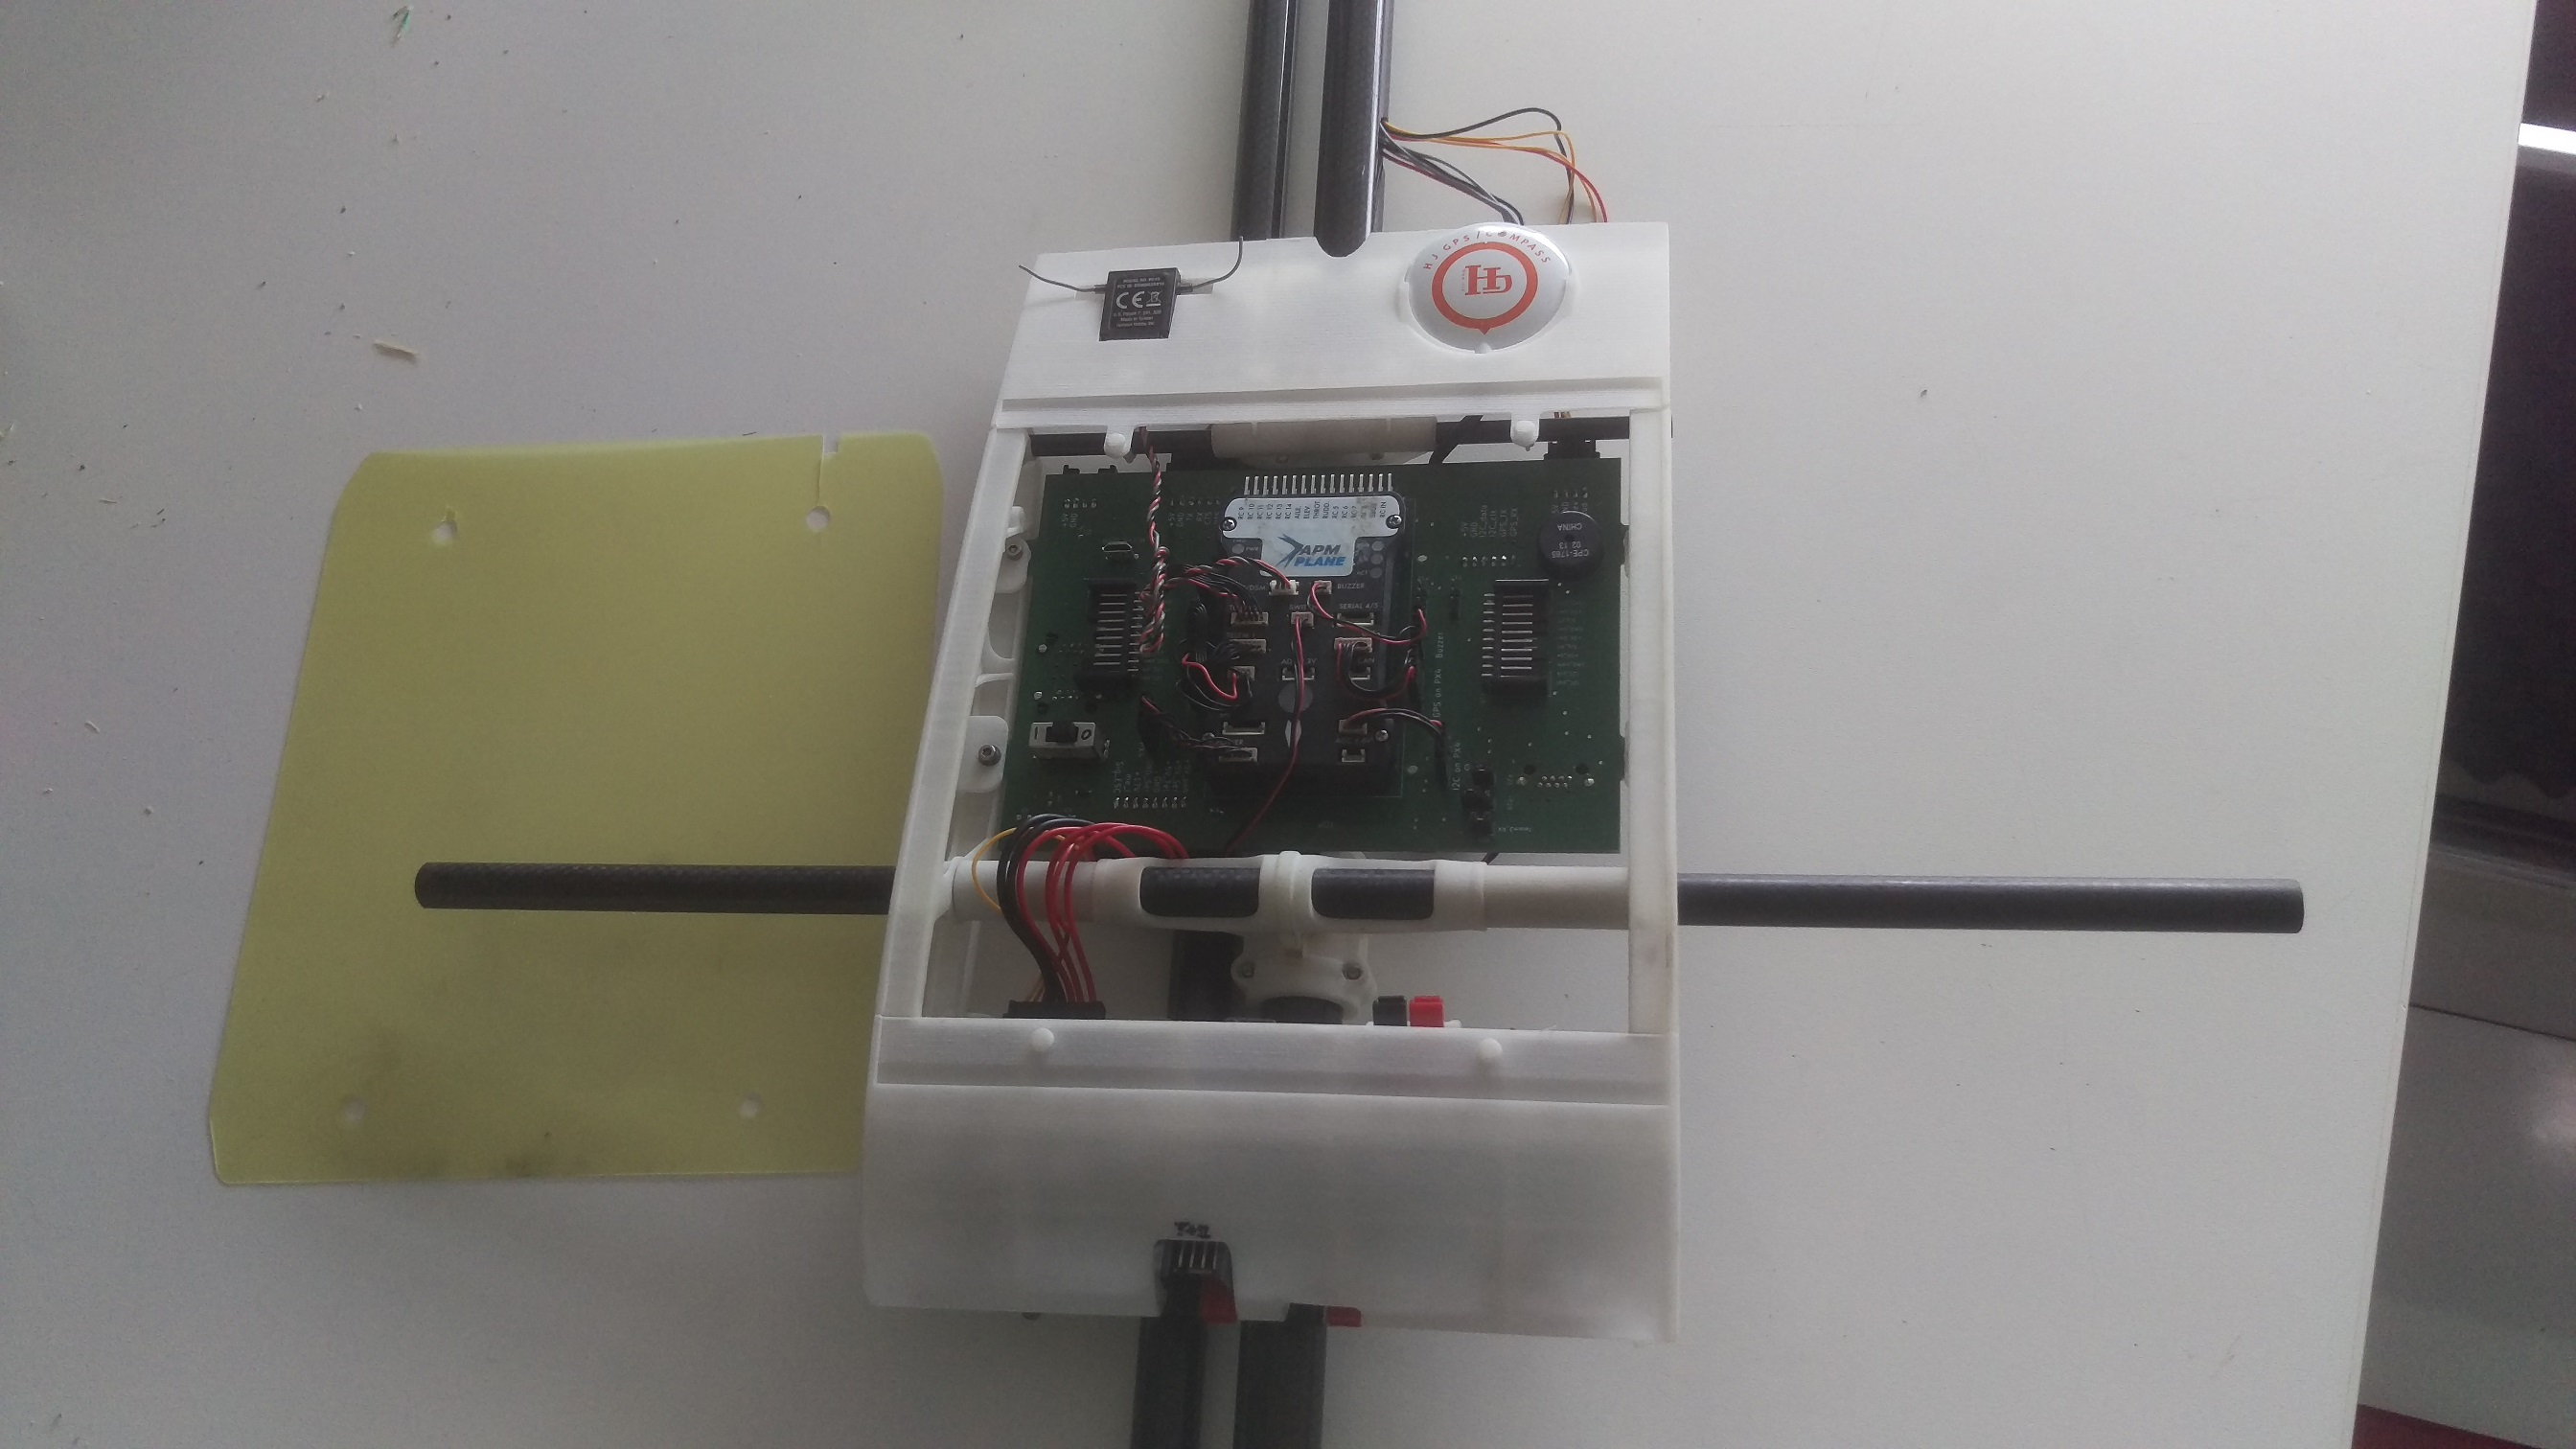
\includegraphics[width=0.9\textwidth]{bilder/Fotos/AUVSI_2016_Centerbox_Detail.jpg} 
\caption{In der WingCenterBox eingebaute Autopilotenplatine} 
\label{fig:In der WingCenterBox eingebaute Autopilotenplatine}
\end{figure}